\section{Background and Related Work}

Figure~\ref{technology} illustrates the fundamentals of the most promising emerging memory technologies to be investigated in our project, namely, the Phase-Change RAM (PCRAM), the Magnetic RAM (MRAM) based on Spin-Torque Transfer RAM(STT-RAM), the resistive RAM (RRAM), and the memristor. In this section, we will briefly describe the physical mechanisms of the emerging NVM devices. The research and development related to this proposal will also be described.

\subsection{Phase-Change RAM (PCRAM)}
PCRAM technology is based on a chalcogenide alloy (typically, Ge$_2$--Sb$_2$--Te$_5$, GST) material, which is similar to those commonly used in optical storage means (compact discs and digital versatile discs)~\cite{Bedeschi09}. The data storage capability is achieved from the resistance differences between an amorphous (high-resistance) and a crystalline (low-resistance) phase of the chalcogenide-based material as shown in Figure~\ref{technology}. In SET operation, the phase change material is crystallized by applying an electrical pulse that heats a significant portion of the cell above its crystallization temperature. In RESET operation, a larger electrical current is applied and then abruptly cut off in order to melt and then quench the material, leaving it in the amorphous state~\cite{burr:scm08}.

PCRAM has shown to offer compatible integration with CMOS technology~\cite{Oh06}, fast speed~\cite{Pirovano03}, high endurance~\cite{Lai03}, and inherent scaling of the phase-change process at 22-nm technology node and beyond~\cite{Chen06}. Compared to STT-RAM, PCRAM is even denser with an approximate cell area of $6\sim12F^2$~\cite{ITRS07}, where F is the feature size. In addition, phase change material has a key advantage of the excellent scalability within current CMOS fabrication methodology~\cite{Cho05,Kim06,Lai01,Pirovano03,Raoux08}, with continuous density improvement~\cite{Nirschl07,Chen07-iedm,Im08}.

Although many device models were built from reliability~\cite{Ielmini07}, low-frequency noise~\cite{Fantini08}, statistical analysis~\cite{Mantegazza07} point of views, they were mainly dedicated to process and device, which cannot be directly borrowed by circuit design and computer community. Many PCRAM prototypes have been demonstrated in the past years by companies like Hitachi~\cite{Hanzawa07}, Samsung~\cite{Lee07-isscc}, STMicroelectronics~\cite{Bedeschi08, Sandre10}, and Numonyx~\cite{Villa10}. The maximum capacities achieved are 1Gb and 256Mb for single level cell (SLC)~\cite{Villa10} and multi-level cell (MLC)~\cite{Lee07-isscc}, respectively. However, to be more competitive to the existing DRAM and Flash memory, PCM need further improvement on density and endurance. In this project, we will address this issue from circuit design point of view.

\begin{figure}
\centering
%\vspace{-10pt}
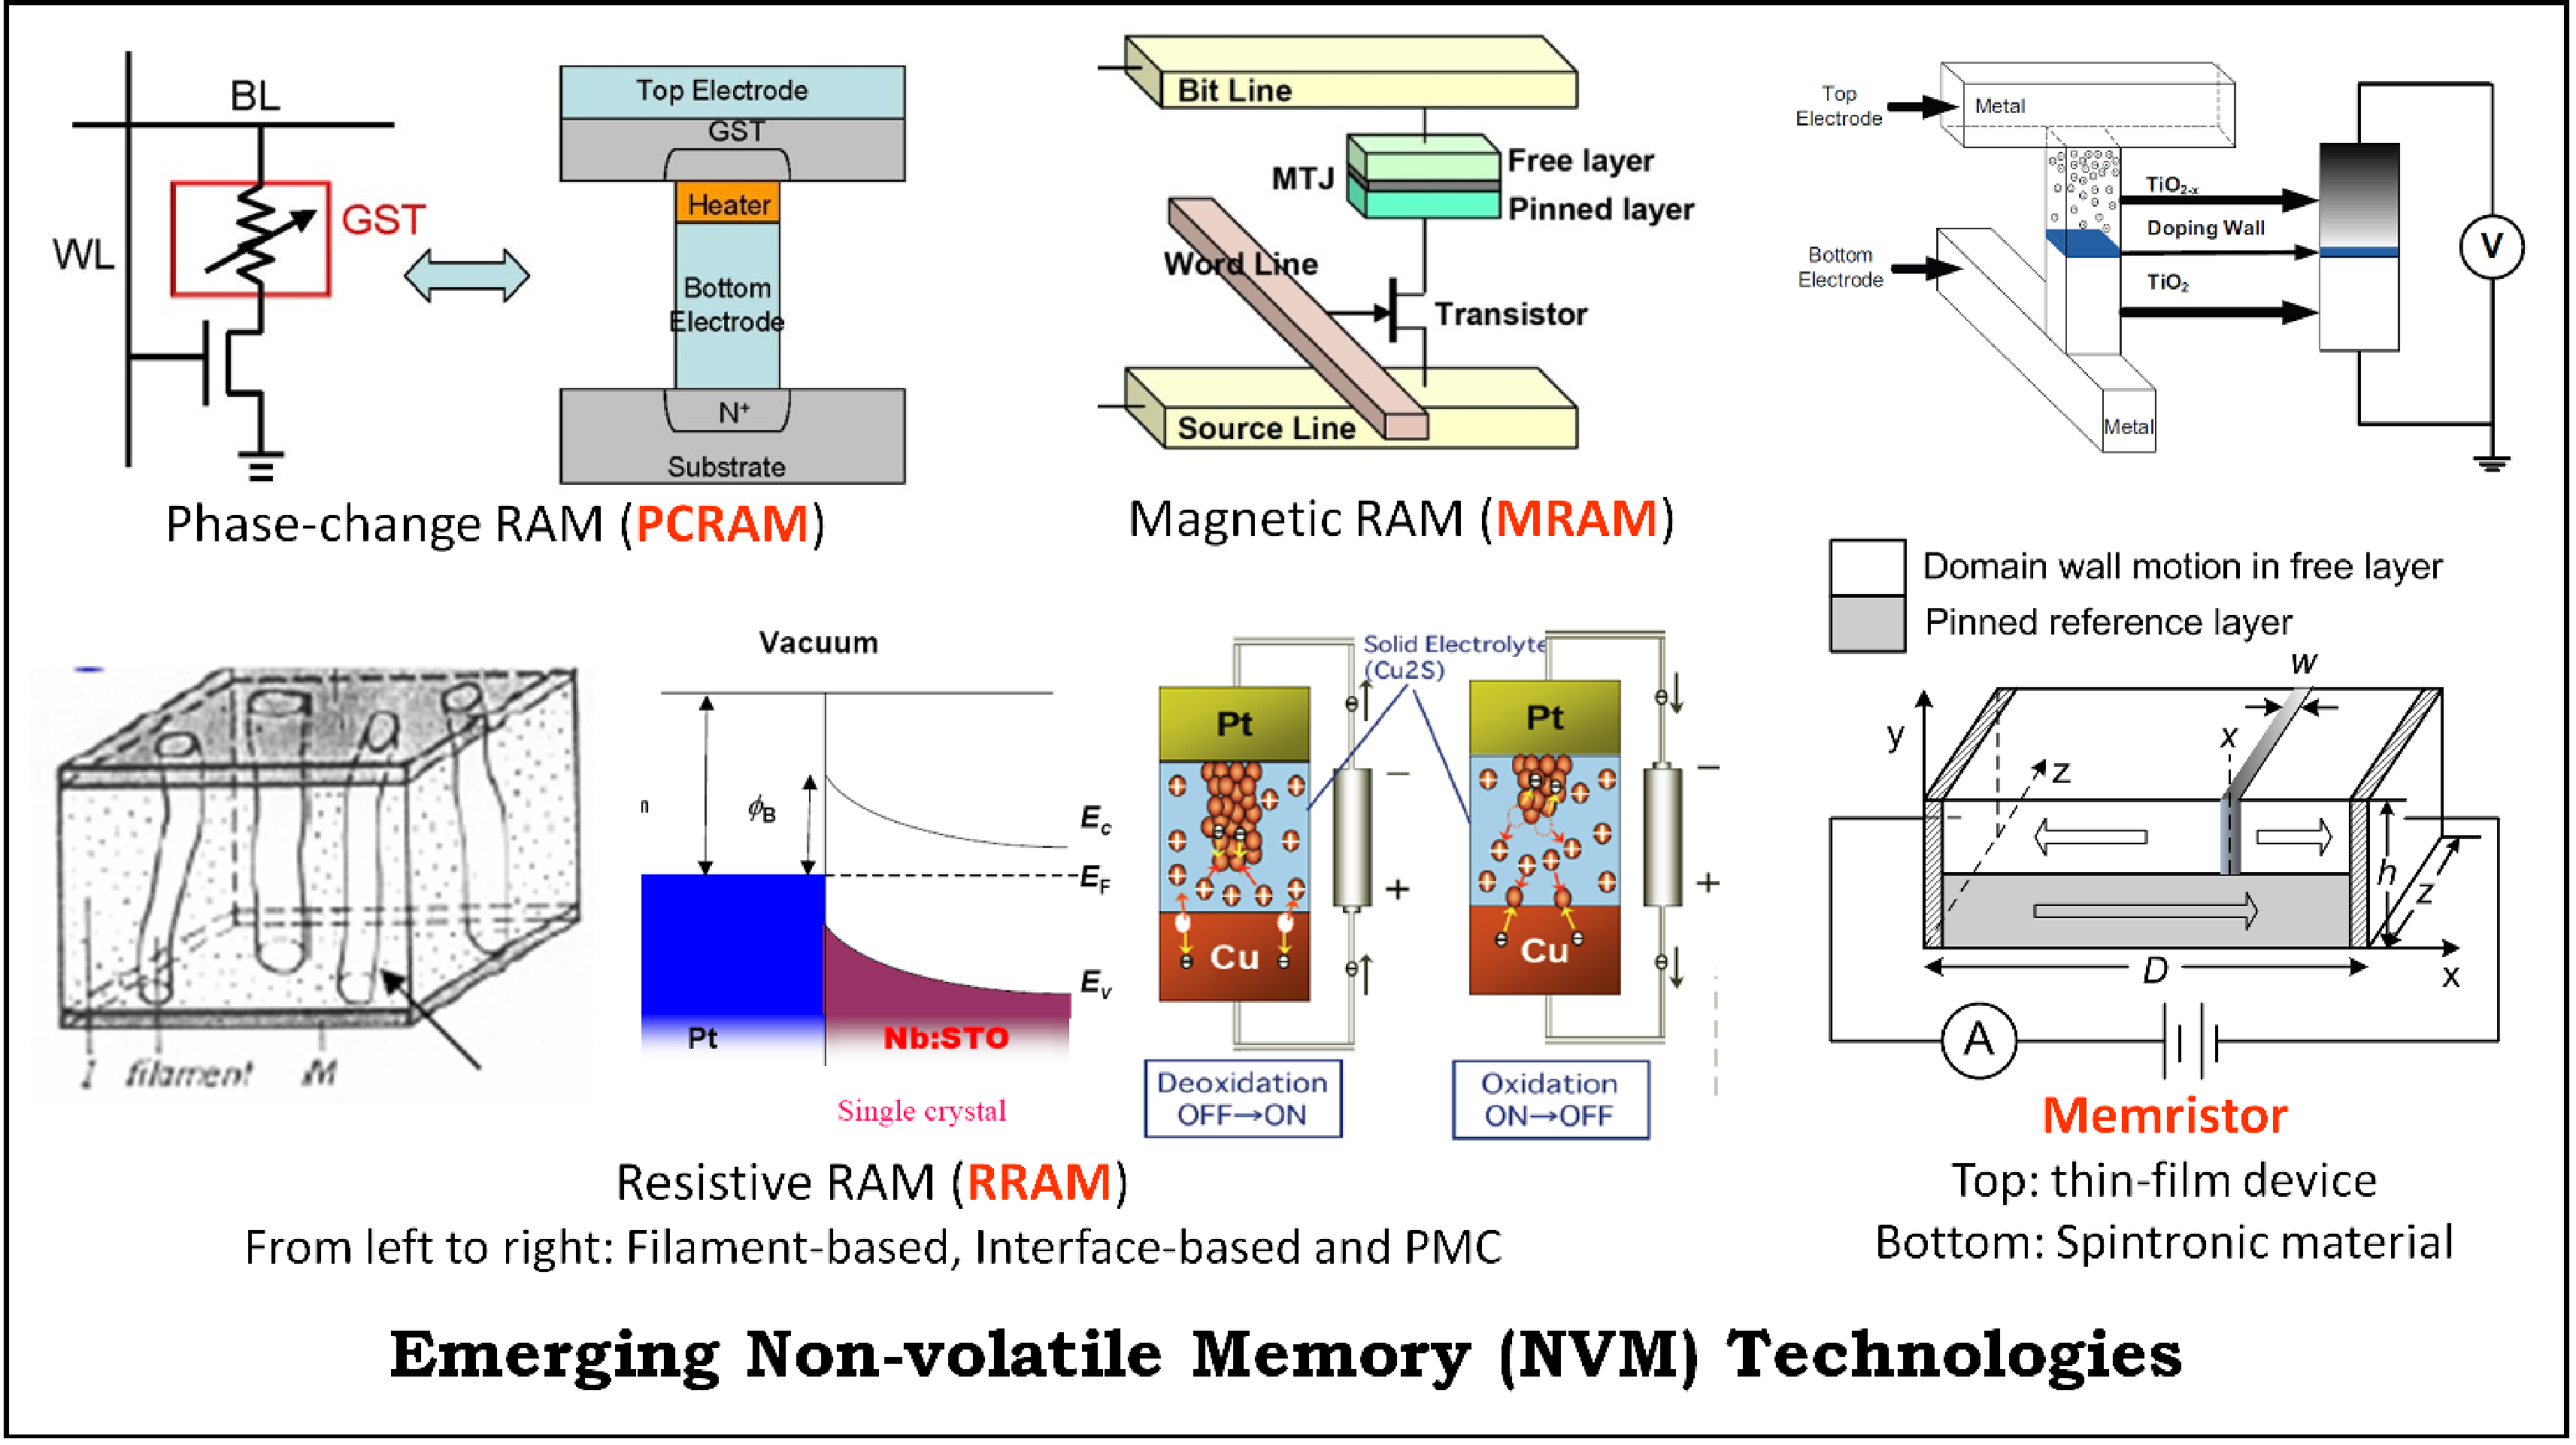
\includegraphics[width=0.95\textwidth]{./figure/1_technology_half.pdf}
\vspace{-10pt}
\caption{\textbf{Overview of Some Emerging Non-volatile Memory Technologies,} including Phase-Change RAM (PCRAM), Magnetic RAM (MRAM), resistive RAM (RRAM), and memristor. }
\label{technology}
\vspace{-10pt}
\end{figure}

\subsection{MRAM based on Spin-Torque Transfer RAM (STT-RAM)}
STT-RAM is a new type of Magnetic RAM (MRAM)~\cite{ITRS07,Hosomi05,MRAM:TTO+06,MRAM:ZBM+06,mram:ibm:maffitt}, which features non-volatility, fast writing/reading speed (\textless 10ns), high programming endurance (\textgreater 10$^{15}$cycles) and zero standby power~\cite{ITRS07}. The storage capability or programmability of MRAM arises from magnetic tunneling junction (MTJ), in which a thin tunneling dielectric, e.g., MgO., is sandwiched by two ferromagnetic layers, as shown in Figure~\ref{technology}. One ferromagnetic layer (``pinned layer'') is designed to have its magnetization pinned, while the magnetization of the other layer (``free layer'') can be flipped by a write event. An MTJ has a low (high) resistance if the magnetizations of the free layer and the pinned layer are parallel (anti-parallel). In first-generation MRAM design, the magnetization of free layer is changed by the current-induced magnetic field~\cite{Motoyoshi04,Ha04}. In STT-RAM, a new write mechanism called ``polarization-current-induced magnetization switching'' is introduced -- the magnetization of free layer is flipped by the electrical current directly. Because the current required to switch an MTJ resistance state is proportional to the MTJ cell area, STT-RAM is believed to have a better scaling property than the first-generation MRAM~\cite{Hosomi05,Kawahara07,MRAM:TTO+06,Diao07,Salahuddin07,Beach08,Kishi08}.

Continuous efforts on process development have been taken on yield improvement~\cite{Miura07}, write power reduction~\cite{Durlam03}, and high density~\cite{Lou08}. Prototyping STT-RAM chips have been demonstrated recently by various companies and research groups~\cite{Hosomi05,Kawahara07,Nebashi09,Motoyoshi04,Andre05,Kawahara08}. Commercial MRAM products have been launched by companies like Everspin (which is a spin-off from Freescale to expedite the technology commercialization in 2008) and NEC.

We have proposed a dynamic MTJ model with more accurate (transient) description for MTJ resistance switching~\cite{Chen08}. Compared to highly conceptual fixed resistance used in traditional STT-RAM design flow, the dynamic model can help to reduce 20\% pessimism in write time at TSMC $0.13{\mu}m$. The failure probability of STT-RAM cells due to parameter variations was considered and discussed in~\cite{Li09}. A model was proposed to predict memory yield and design optimization to minimize memory failures. MRAM potentially could be next-generation on-chip cache or memory due to its fast access and soft-error resistance. We will work toward this direction and look for new solutions and more applications to fast this procedure.

\subsection{Resistive RAM (RRAM)}
In an R-RAM cell, the data is stored as two (single-level cell, or SLC) or more resistance states (multi-level cell, or MLC) of the resistive switch device (RSD). Resistive switching in transition metal oxides was discovered in thin NiO film decades ago~\cite{Gibbons64}. From then, a large variety of metal-oxide materials have been verified to have resistive switching characteristics, including TiO$_2$~\cite{Fujimoto06}, NiO$_x$~\cite{Jung07}, Cr-doped SrTiO$_3$~\cite{Janousch07}, PCMO~\cite{Liu00}, and CMO~\cite{Hsu07} etc. Based on the storage mechanisms, RRAM materials can be cataloged as filament-based, interface-based, programmable-metallization-cell (PMC), etc. Based on the electrical property of resistive switching, RSDs can be divided into two categories: unipolar or bipolar.

Filament-based RRAM is a typical example of unipolar switching~\cite{Inoue} that has been widely investigated. The insulating material between two electrodes can be made conducting through a hopping or tunneling conduction path after the application of a sufficiently high voltage. %a process called electro-forming. 
The data storage could be achieved by break (RESET) or reconnect (SET) the conducting path. Programmable-metallization-cell (PMC)~\cite{Kozicki05} is a promising bipolar switching technology. The switching mechanism of PMC can be explained as forming or breaking the small metallic ``nanowire'' by moving the  metal ions between two sold metal electrodes.

\textbf{\underline{HL: Related work.}}

\subsection{Memristor}
Memristor, the fourth fundamental passive circuit element, was predicted by Professor Chua in 1971~\cite{Chua71}, based on the completeness of circuit theory. %Different from other electrical parameters resistance (\textit{R}), capacitance (\textit{C}) and inductance (\textit{L}), 
Memristance (\textit{M}) is a function of charge (\textit{q}),  which depends upon the historic behavior of the current (or voltage) profile~\cite{Chua76,Strukov08}. In 2008, 37 years after memristor was predicted in theory, the researchers at HP reported the first real device of a memristor. The memristive effect was achieved in a solid-state thin film two-terminal device by moving the doping front along the device as shown in Figure~\ref{technology}~\cite{Tour08}. Afterwards, magnetic technology provides the other possible methods to build a memristive system~\cite{Pershin08,Wang09}. Due to its unique historic characteristic, memristor has very broad application including nonvolatile memory, signal processing, control and learning system etc~\cite{Chen09}.

\textbf{\underline{HL: Related work.}} Indeed, HP Labs plan to unveil RRAM prototype chips based on memristor with crossbar arrays soon.

\begin{figure}
\centering
\vspace{-10pt}
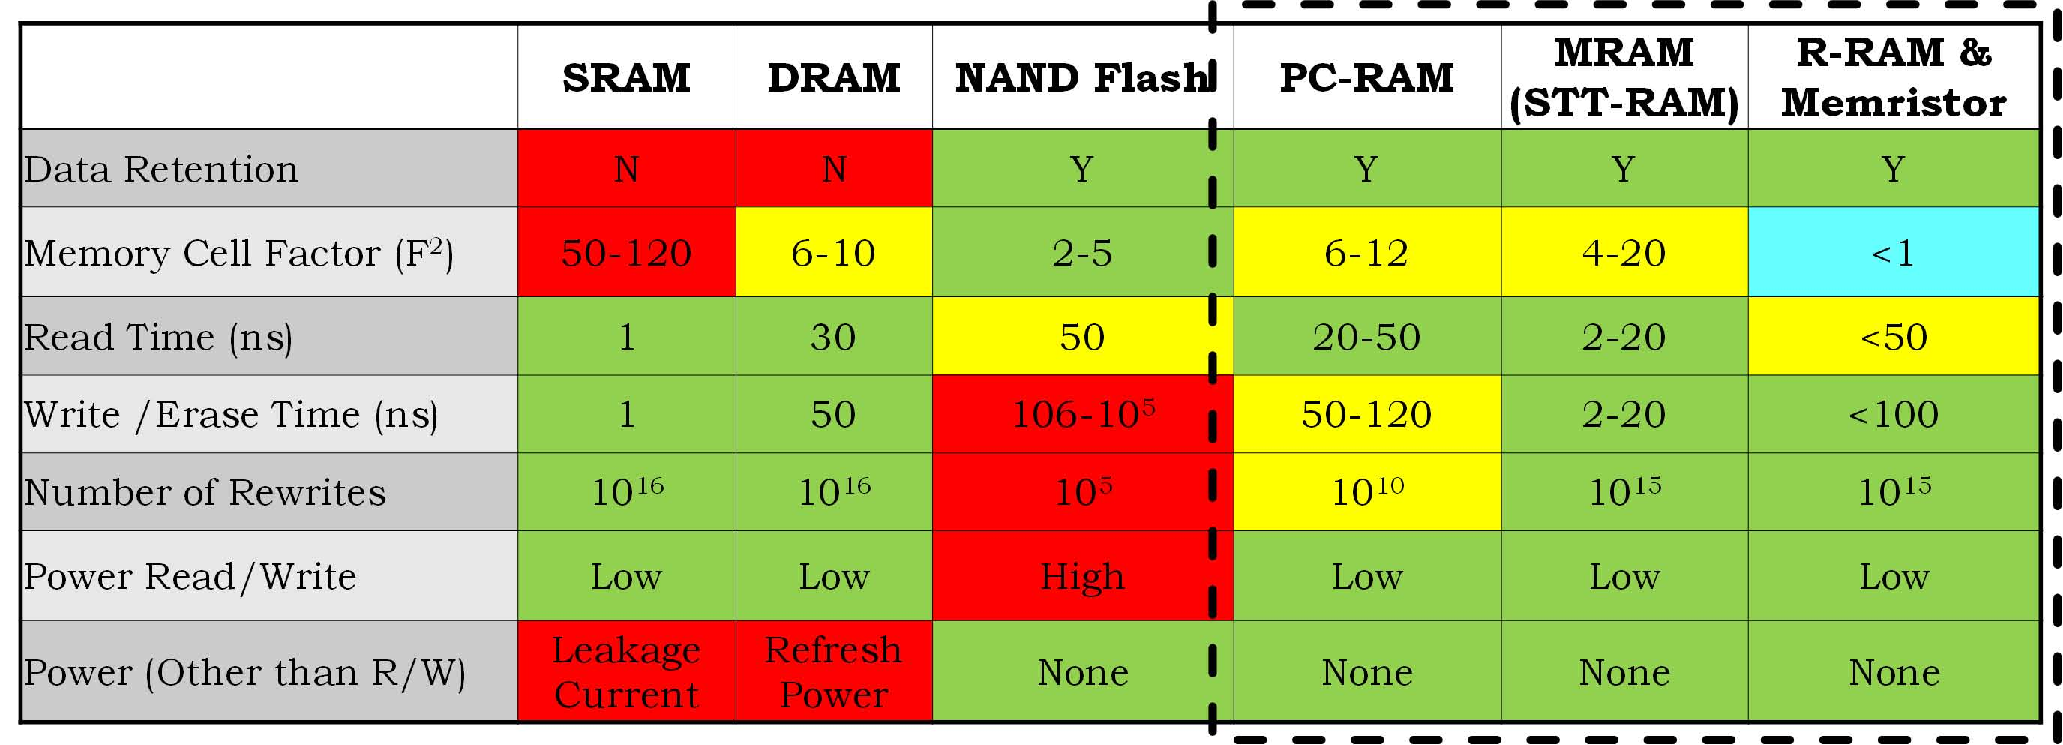
\includegraphics[width=0.9\textwidth]{./figure/2_table.pdf} 
\vspace{-10pt}
\caption{The comparison of various memory technologies~\cite{ITRS07}.}
\label{table}
\vspace{-10pt}
\end{figure}

\paragraph{Summary}
Figure~\ref{table} illustrates the comparison of emerging memory technologies -- PCRAM, MRAM (STT-RAM), RRAM and Memristor -- against the traditional main-stream SRAM, DRAM, and NAND-based Flash memory~\cite{ITRS07}. Note that both CMOS-compatible embedded MRAM (NEC)~\cite{MRAM:NEC09} and embedded PCRAM (Hitachi and STMicro)~\cite{Hanzawa07,PRAM:ST2004} have been demonstrated, paving the way of integrating these NVMs to the traditional memory hierarchies. In addition, the emerging 3D integration technologies~\cite{xie:jetcs06,Xie:dac08} enables cost-effective integration of these NVMs with CMOS logic circuits. With all the NVM technology advances in recent years, it is anticipated that the emerging NVM technologies will break important ground and move closer to market in the near future (``Non-volatile memory goes commercial", EEtimes, 12/02/2009).


